% $Header: /cvsroot/latex-beamer/latex-beamer/examples/beamerexample3.tex,v 1.8 2004/10/07 20:53:07 tantau Exp $


%\documentclass[handout]{beamer}
\documentclass{beamer}

% Copyright 2003 by Till Tantau <tantau@cs.tu-berlin.de>.
%
% This program can be redistributed and/or modified under the terms
% of the LaTeX Project Public License Distributed from CTAN
% archives in directory macros/latex/base/lppl.txt.

%
% The purpose of this example is to show how \part can be used to
% organize a lecture.
%

\usetheme{Boadilla}
\usepackage[english]{babel}
\usepackage[latin1]{inputenc}

\setbeamercovered{transparent}
\setbeamertemplate{navigation symbols}{}

%\usepackage{pgfpages}
%\pgfpagelayout{4 on 1}[a4paper,landscape,border shrink=5mm]

%
% The following info should normally be given in you main file:
%


\title{Simulations for Touschek Lifetime}
\author{Helge Kr\"uger}
\institute{University of Vienna}
%\logo{\includegraphics[heihgt=0.1cm]{PSIlogoBW.pdf}}

\begin{document}


\frame{\titlepage}

\section*{Outlines}

\frame{
  \frametitle{Outline of the Talk}

  \begin{block}{About me}
  I'm Helge Kr\"uger. I study Physics at the University of Vienna.\\
  In this talk, I want to talk about what I did as a summer student at the Paul Scherrer Institut in the summer 2005.
  \end{block}
  \pause

  \begin{block}{Outline of the talk}
  \begin{itemize}
   \item What is the Touschek effect?
   \item Modeling, Programming and Validation of the Effect.
   \item Simulations for the SLS and low emittance studies.
   \item Conclusions/Future 
  \end{itemize}
  \end{block}
}

\part{What is the Touschek Effect?}
\frame{
 \partpage  
 \tableofcontents[part=1]
}


\section{What is the Touschek Effect?}
\frame{
  \frametitle{What is the Touschek Effect?}
  \begin{block}{The Touschek Effect}
  \begin{itemize}
  \item Discovered 1963 in Orsay
  \item Interpreted by B. Touschek.
  \end{itemize}
  \end{block} \pause
  \begin{block}{How it works}
  \begin{itemize}
   \item Electrons in the beam of a storage ring interact through the Coulomb force.
   \item Transversal momentum is transferred to longitudinal momentum.
   \item The momentum increase is multipplied by $\gamma$ (relativistic effect) 
   \item If the longitudinal momentum becomes larger then the momentum acceptance, the electrons are lost. 
  \end{itemize}
  \end{block}
}

\section{Calculations for the Lifetime}
\subsection{A First Formula for the Lifetime}
\frame{
  \frametitle{A First Formula for the Lifetime}
  \begin{block}{Assumptions}
  \begin{itemize}
  \item The bunch has N electrons.
  \item Each electron can interact with every other electrons. (Possible interactions $\propto N^2$)
  \item The number of lost electrons is proportional to the number of possible interactions.
  \end{itemize}
  \end{block}\pause
  \begin{block}{Conclusions}
  \begin{equation} \dot N = - \alpha N^2 \end{equation}
  With $\alpha$ a factor to be determined. 
  For the lifetime we have:
  \begin{equation} \tau_{1/2} = \frac 1 { \alpha \cdot N} \end{equation}
%  \begin{equation} \tau_{1/2} = \left( \alpha \cdot N \right)^{-1} \end{equation}
  \end{block}
}

\subsection{Analytic Approaches}
\frame{
  \frametitle{Analytic Approaches}
  \begin{block}{Calculating $\alpha$}
  \begin{itemize}
   \item Bruck, V\"olkel, ... derived formulas for $\alpha$.
   \item Used assumptions as non-relativistic motion, no vertical motion, all particles have same energy.
  \end{itemize}
 % As an example we have:
 %   \begin{equation} \alpha = \frac{r_0 ^2 c}{8 \pi \gamma^3 \sigma_s} \frac{F\left(\left(\delta_{acc} / \gamma \sigma_{x'}\right)^2\right)}{\sigma_x \sigma_y \sigma_{x'} \delta_{acc} ^2} \end{equation} 
 % To derive this people used different assumptions, as non-relativistic motion, all particles have same energy or no vertical motions
  \end{block} \pause
  \begin{block}{Example of a formula}	
  \begin{equation} \alpha = \frac{r_0 ^2 c}{8 \pi \gamma^3 \sigma_s} \frac{F\left(\left(\delta_{acc} / \gamma \sigma_{x'}\right)^2\right)}{\sigma_x \sigma_y \sigma_{x'} \delta_{acc} ^2} \end{equation} 
  \begin{itemize}
  \item $\delta_{acc}$ the momentum acceptance.
  \item $\sigma_x$ the standard deviation of the bunch size.
  \item $\sigma_{x'} = \frac{\epsilon_x}{\sigma_x} \sqrt{1 + H \cdot \frac{\sigma_{s'} ^2}{\epsilon_x}}$ is the rms divergence of the $p / p_0$ at $x = 0.$
  \item $F(x) = \int\limits_0^1 \left(\frac 2 u - \ln \frac 1 u -2\right) e^{-x / u} du$
  \end{itemize}

  \end{block}

%  \begin{block}{Our use}
%  \begin{itemize}
%  \item We use these formulas to test our model.
%  \item And we can draw conclusions on how the Touschek Lifetime scales with the parameters.
%  \end{itemize}
%  \end{block}
}

\section{Monte Carlo Simulations by S. Khan}
\frame{
  \frametitle{Monte Carlo Simulations by S. Khan}
  \begin{block}{Idea behind the Monte Carlo Integration}
  Evaluate the following Integral giving the number of lost electrons.
  \begin{equation} \dot N = \frac{1}{\gamma C} \oint ds \int d\vec R \int d\vec P \int d\vec P' \int d\Omega \  2 v \sigma \sin \Theta \rho_1 \rho_2 \end{equation}
  \begin{itemize}
  \item s is the integral along the storage ring
  \item $\vec R$ space coordinate where the interaction takes place
  \item $\vec P, \vec P'$ momenta coordinates of the interacting electrons
  \item $\sigma$ the M{\o}ller cross section
  \item v the relative speed
  \item $\Theta$ the scattering angle
  \item $\rho_1$, $\rho_2$ the particle densities
  \item $1/\gamma$ to transform from bunch to laboratory system
  \end{itemize}
  \end{block}
}

\subsection{Evaluation of the Integral}
\frame{
  \frametitle{Evaluation of the Integral}
  \begin{block}{Evaluation of the Integral}
  \begin{itemize}
   \item Pick out a place for the interaction to take place. (s and $\vec R$ coordinate)
   \item Pick out 2 momenta coordinates ($\vec P, \vec P'$) for the colliding electrons, and 2 scattering angles ($\Theta, \Phi$).
   \item Do the scattering of the electrons using relativistic kinematics.
   \item If outside momentum acceptance, compute using the number the percentage of electrons.
   \item Calculate $\alpha$ summing over all events in:
   \begin{equation} \alpha \approx \frac{\Delta V}{n} \frac 1 {\gamma C} \sum\limits_{Events} 2 v \sigma \sin \Theta \rho_1 \rho_2 \end{equation}
   \end{itemize}
   \end{block}
}

\part{Modeling}
\frame{
 \partpage  
 \tableofcontents[part=2]
}

\section{Modeling the Coulomb Interactions}
\frame{
  \frametitle{Modeling the Coulomb Interactions}

  \begin{block}{Direct Monte Carlo Simulation + Particle Tracking}
  \begin{itemize}
   \item Linear beam optics move the electrons around.
   \item Find the electrons that are close. 
   \item Let them interact, analytically determining the scattering angle.
   \item Take out electrons out of momentum acceptance.
  \end{itemize}
  \end{block}\pause

  \begin{block}{This failed, because:}
  \begin{itemize}
   \item High use on computing power: Computation of nearest neighbors, high number of particles needed for statistics.
   \item Modeling 2 particle interactions.
  \end{itemize}
  \end{block}
}

\section{What we do now!}
\frame {
  \frametitle{What we do now!}
  \begin{block}{Idea similar to S. Khan combined with particle tracking}
    \begin{itemize}
  \item Particles with coordinates $\xi \in \mathbb{R}^6$.
  \item Linear Beam Optics, to move the particles \\ $\xi_f = M \cdot \xi_i$ with $M \in \mathbb{R}^{6 \times 6}$.
  \item For each particle in our bunch, we do the interaction.
  \item Interaction partner is a particle assumed at the same place, and with a random momentum.
  \item Interaction is done using relativistic kinematics and random scattering angles.
  \end{itemize}
  \end{block} 
  \pause
  \begin{block}{Calculating the Touschek Lifetime}
  \begin{itemize}
  \item With the M{\o}ller cross section.
  \item Densities in phase space.
  \end{itemize}
  \end{block}
}

\subsection{Relativistic Kinematics}
\frame {
  \frametitle{Relativistic Kinematics}
  \begin{block}{Transformations}
  \begin{itemize}
  \item Coordinates for particle tracking in laboratory system.
  \item Transformed to the center of momentum system of the 2 interaction partners.
  \end{itemize}
  \end{block} \pause
  \begin{block}{The Interaction}
  \begin{itemize}
  \item 2 random scattering angles $\Theta$ and $\Phi$.
  \item Rotation of the momentum in c.m.s. around these angles.
  \end{itemize}
  \end{block} \pause
  \begin{block}{Backtransform and Acceptance}
  \begin{itemize}
  \item Transform back to laboratory system.
  \item Check if outside momentum acceptance, if yes count as event.
  \end{itemize}
  \end{block}
}
\subsection{M{\o}ller cross section}
\frame {
  \frametitle{M{\o}ller-Cross section}
  \begin{block}{The M{\o}ller-Cross section from Quantum Electrodynamics}
  \begin{equation} \sigma = \frac{r_e ^2}{4} \left(1 - \frac{v^2}{c^2}\right) \left[ (X+1)^2 \left(\frac 4 {\sin^4 \Theta} - \frac 3 {\sin^2 \Theta}\right) + 1 + \frac 4 {\sin^2 \Theta}\right] \end{equation}  
  With $X = (c/v)^2$. This cross section is valid in the center of momentum frame, and doesn't take into account beam polarization.
  \end{block} 
  \begin{columns}\begin{column}[t]{3cm}
   \begin{figure}[here]
   \centering

     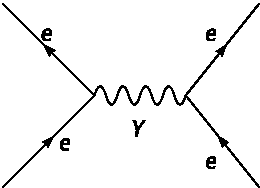
\includegraphics[width=1.00\textwidth]{inter.pdf}
     \caption{The Interaction}
   \end{figure} \pause
  \end{column}
  \begin{column}[t]{8cm}
  \begin{block}{Number of lost particles in one interaction}
  \begin{equation} \Delta n = 2 v \sigma \sin \Theta \rho_1 \rho_2 \end{equation}
  \begin{itemize}
  \item $\Delta n$ number of lost particles
  \item v relative speed
  \item $\rho_1, \rho_2$ particle densities
  \end{itemize}
  \end{block}
  \end{column}\end{columns}
}
\subsection{Computation of $\alpha$}
\frame {
  \frametitle{Computation of $\alpha$}
  \begin{block}{Our simulation}
  \begin{itemize}
  \item For each particle $(\vec R_i, \vec P_i)$ in the simulated bunch, pick out a momentum $\vec P'$ for a particle to interact with, and 2 scattering angles $\Theta$ and $\Phi$.
  \item Check if the particle would go outside momentum acceptance, if yes count this event.
  \end{itemize}
  \end{block} \pause
  \begin{block}{$\alpha$ is given by:}
  \begin{equation} \alpha = \frac{\Delta V}{n} \frac 1 {C \gamma} \sum\limits_{Events} 2 v \sigma \sin \Theta \rho_2 \end{equation}
  v and $\sigma$ are in the bunch system. $\rho_2 = \rho(\vec R_i, \vec P')$
  The particles in the bunch are already gaussian distributed, so we have no $\rho_1$.\\
  C is the circumference of the storage ring.\\
  $\Delta V$ is the volume, where we pick our random values out.
  \end{block}
}

%\subsection{Different Approaches to Computation}
%\frame{
% \frametitle{Different Approaches to Computation}
% \begin{block}{We need} \begin{itemize}
% \item one position $\vec R$
% \item two momenta $\vec P, \vec P'$
% \item two scattering angles $\Theta, \Phi$ (always random)
% \end{itemize}
% \end{block} \pause
% \begin{block}{Ways to chose interaction partners}
% \begin{itemize}
% \item {\bf Analytic} Chose 1 coordinate and 2 momenta at random.
% \item {\bf Semianalytic} Take one particle out of the bunch, and momentum for colliding particle at random.
% \item {\bf 2 Particles} Take 2 particles out of the bunch, and use momentum of second particle as momentum of the colliding particle.
% \end{itemize}
% \end{block} \pause
% \begin{block}{Differences between the approaches}
% \begin{itemize}
% \item Analytic and semianalytic give about to the same result ($\pm 20 \%$)
% \item 2 Particles gives up to 3 orders of magnitude wrong. Using nearest neighbors could fix this.
% \end{itemize}
% \end{block}
%}

\subsection{Differences to S.Khan's Simulation}
\frame{
 \frametitle{Differences to S.Khan's Simulation}
 \begin{columns}  \begin{column}[t]{5.5cm}
 \begin{block}{S.Khan's Simulation}
 \begin{itemize}
 \item Monte Carlo Integration.
 \item Beam parameters given.
 \item No particle tracking.
 \item Place, both momenta and angles are random.
 \item 12 dimensional random volume.
 \end{itemize}
 \end{block}
 \end{column} \pause  \begin{column}[t]{5.5cm}
 \begin{block}{My Simulation}
 \begin{itemize}
 \item Particle tracking with linear optics
 \item Beam parameters computed out of tracked particles
 \item Only scattering angles and momentum of interaction partner are random
 \item 5 dimensional random volume.
 \end{itemize}
 \end{block}
 \end{column}\end{columns} \pause
 \begin{block}{Theoretical models}
 \begin{itemize}
 \item More assumptions about beam geometry
 \item Not fully relativistic.
 \end{itemize}
 \end{block}
}

\section{Implementation}
\frame{
 \frametitle{Implementation: The Touschek Tracker (ttrack)}
 \begin{columns}
 \begin{column}[t]{5cm}
  \begin{block}{What was used:}
  \begin{itemize}
  \item C/C++ for program code
  \item $IP^2L$ (Independant Parallel Particle Layer) library for particle tracking
  \item Supercomputer Horizon: Cray XT-3
  \item Parallel processing
  \end{itemize} 
  \end{block} \pause
  \begin{block}{Possibilities}
  \begin{itemize}
  \item Different Lattices
  \item 6D Distributions
  \end{itemize}
  \end{block} \pause
 \end{column}
 \begin{column}[t]{6cm}
  \begin{block}{Scaling}  
   \begin{figure}[here]
   \centering
     \includegraphics[width=1.00\textwidth]{scaling.pdf}
    \caption{Scaling of ttrack}
   \end{figure}
  \end{block}
 \end{column}
 \end{columns}
}


\part{Simulation and Measurements}
\frame{
 \partpage  
 \tableofcontents[part=3]
}

\section{Simulation for Aurora and Comparison with theory}
\frame {
  \frametitle{Simulation for Aurora and Comparison with theory}
  \begin{columns}\begin{column}[t]{5cm}
  \begin{block}{What we did}
  \begin{itemize}
  \item Aurora is a simple magnet: fully symmetric except for the cavity.
  \item Predictions for lifetime from analytical formulas
  \item Compare this to our program.
  \end{itemize}
  \end{block}  \pause
  \begin{block}{Conclusions}
  \begin{itemize}
  \item The value predicted by the simulation, is in $\pm 5 \%$ from different formulas.
  \end{itemize} \end{block}
  \end{column}\begin{column}[t]{6cm}
  \begin{block}{Results}
  \begin{figure}[here]
  \centering
    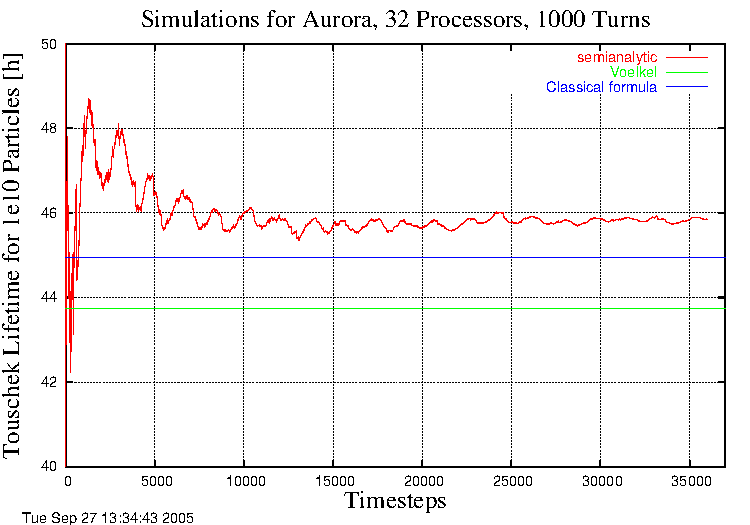
\includegraphics[width=1.00\textwidth]{aurlong.pdf}
   \caption{Simulation for Aurora}
  \end{figure} \end{block} 
  \end{column}\end{columns}
}

\section{Simulations for SLS}
\frame {
  \frametitle{Simulations for SLS}
  \begin{columns}\begin{column}[t]{5cm}
  \begin{block}{What we did}
  \begin{itemize}
%  \item SLS a sample case to compare simulation with experiment
  \item Simulation of a third of the machine with linear optics
  \item Bunch of $6 \cdot 10^9$ Particles, 1 mA
  \item Momentum acceptance changed in measurements using a scraper
  \end{itemize}
  \end{block}  \pause
%  \begin{block}{Possible error causes}
%  \begin{itemize}
%  \item Not knowing well position of scraper.
%  \item Problems with simulations (see later)
%  \item Assumptions about beam geometry % (e.g. $\epsilon_y = 0.01 \cdot \epsilon_x$)
%  \end{itemize}
%  \end{block}\pause
  \end{column}\begin{column}[t]{6cm}
  \begin{block}{Results}
  \begin{figure}[here]
  \centering
    \includegraphics[width=1.00\textwidth]{sls-acceptance.pdf}
   \caption{SLS-Acceptance vs. Touschek Lifetime}
  \end{figure} \end{block} 
  \end{column}\end{columns}
%  \begin{tabular}{l|l}
%  Momenta Acceptance & Touschek Lifetime \\ \hline
%  0.5 \% & 0.12 h \\
%  1.0 \% & 1.01 h \\
%  1.5 \% & 3.70 h \\
%  2.0 \% & 8.71 h 
%  \end{tabular}
}


\subsection{Reasons for big difference}
\frame{
 \frametitle{Reasons for big difference}
 \begin{columns}
 \begin{column}[t]{6cm}
  \begin{block}{Results}
  \begin{figure}[here]
  \centering
    \includegraphics[width=1.00\textwidth]{sls-acceptance.pdf}
   \caption{SLS-Acceptance vs. Touschek Lifetime}
  \end{figure} \end{block} 
  \end{column} \begin{column}[t]{5cm} 
  \begin{block}{Possible error causes}
  \begin{itemize}
  \item Simulation has global acceptance
  \item Measurement has local acceptance
  \item Measurement and simulation are not comparable
  \item Need to change momentum acceptance using the RF Cavity.
  \end{itemize}
  \end{block}
%  \begin{block}{Reasons for smaller errors}
%  \begin{itemize}
%  \item Not knowing well position of scraper.
%  \item Assumptions about beam geometry \\ (e.g. $\epsilon_y = 0.01 \cdot \epsilon_x$)
%  \item Residual gas scattering shortening the lifetime
%  \item Nonlinear effects changing the bunch shape.
%  \end{itemize}
%  \end{block}
  \end{column} \end{columns}
}

\subsection{Linear Behavior}
\frame{

 \frametitle{Linear Behavior}
 \begin{columns}
 \begin{column}[t]{6cm}
  \begin{block}{Results}
  \begin{figure}[here]
  \centering
    \includegraphics[width=1.00\textwidth]{linbehavior.pdf}
   \caption{Checking}
  \end{figure} \end{block} 
  \end{column} \begin{column}[t]{5cm} 
  \begin{block}{What are we doing?}
  \begin{itemize}
  \item Touschek lifetime given by:
  \begin{equation} \tau = \frac 1 {\alpha N} \end{equation}
  \item We check it
  \end{itemize}
  \end{block} \pause
  \begin{block}{Interpretation}
  \begin{itemize}
  \item Up to 1 mA, the linearity is given
  \item After 1 mA, it is no longer true, due to effects like bunch lengthening caused by its own charge.
  \end{itemize}
  \end{block}
  \end{column} \end{columns}
}

\section{Low Emittance Studies}
\frame {
  \frametitle{Low Emittance Studies for SLS}
  \begin{columns}\begin{column}[t]{5cm}
  \begin{block}{Why do this?}
  \begin{itemize}
  \item Classical formulas predict lifetime becoming longer again with ultra low emittance.
  \item This was never tested by experiment.
  \item Computer simulation is a way to validate this.
  \end{itemize}
  \end{block} \pause
  \begin{block}{Scaling}
  \begin{eqnarray}
  \epsilon &\rightarrow& \epsilon / F \\
  \sigma &\rightarrow& \sigma / \sqrt F
  \end{eqnarray}
  \end{block} \pause
  \end{column}\begin{column}[t]{6cm}
  \begin{block}{Results}
  \begin{figure}[here]
  \centering
    \includegraphics[width=1.00\textwidth]{emi.pdf}
   \caption{Low Emittance Studies}
  \end{figure}
  \end{block} 
  \end{column}\end{columns}
%  \begin{block}{Results, also on next figure}
%  \begin{itemize}
%  \item Using $\epsilon \rightarrow \epsilon / F$ with $F \geq 1$
%  \item Lifetime first goes down.
%  \item At F = 50'000 lifetime is back at the same as F = 1.
%  \item Then lifetime goes up fast.
%  \end{itemize}
%  \end{block}
}

\subsection{Aurora}
\frame {
  \frametitle{Low Emittance Studies for Aurora}
  \begin{columns}\begin{column}[t]{6cm}
  \begin{block}{Results}
  \begin{figure}[here]
  \centering
    \includegraphics[width=1.00\textwidth]{emiaur.pdf}
   \caption{Low Emittance Studies}
  \end{figure}
  \end{block}
  \end{column}\begin{column}[t]{5cm}
  \begin{block}{Conclusions}
  \begin{itemize}
  \item Lifetime goes back up earlier then the classical formula predicts
  \item Classical formula is accurate for scaling up to a factor of $10^4$.
  \item For $F > 10^4$ lifetime grows back faster after the classical formula.
  \end{itemize}
  \end{block}
  \end{column}\end{columns}
}

\part{Conclusions and Future}
\frame{
 \partpage  
 \tableofcontents[part=4]
}

\section{Summary of what we did}
\frame{
  \frametitle{Summary of what we did}
  \begin{block}{Writing a program}
  \begin{itemize}
  \item Working program to compute Touschek Lifetimes.
  \item Input Linear Lattice and matched beam.
  \item Output value for $\alpha$. Touschek Lifetime can be calculated knowing bunch charge.
  \end{itemize}
  \end{block} \pause
  \begin{block}{Running simulations}
  \begin{itemize}
  \item Simulated the SLS and compared with measurements.
  \item Checked that lifetime goes back up at very low emittance.
  \end{itemize}
  \end{block}

}

\section{What is still to do}
\frame {
  \frametitle{What is still do?}
  \begin{block}{Things to be changed}
  \begin{itemize}
  \item Include synchrotron radiation, non-linear optic effects, scattering of residual gas, etc...
  \item Model loss of particles, by for example giving each particle a weight $Q_i$ and removing from it on each scattering.
  \item Use 2 particle from the bunch, instead of picking out a random number, maybe by always using the nearest neighbor as interaction partner. 
  \item Use a mesh to compute the densities of the particles (6D mesh in Phase space).
  \item Retry doing it computing the scatterings using the Coulomb force to determine how the interaction happens.
  \item Various other things, you will find in the report.
  \end{itemize}
  \end{block}
}

\section{Comments? Open Questions?}
\frame{
 \frametitle{Comments? Open Questions?}
 \begin{block}{More Information}
 Try looking at the SLS-Notes for my report\\
 http://slsbd.psi.ch/pub/slsnotes/
 \end{block}
}


\appendix

\section{Long term Behavior}
\frame {
  \frametitle{Long term Behavior Semianalytic vs Analytic}
  \begin{figure}[here]
  \centering
    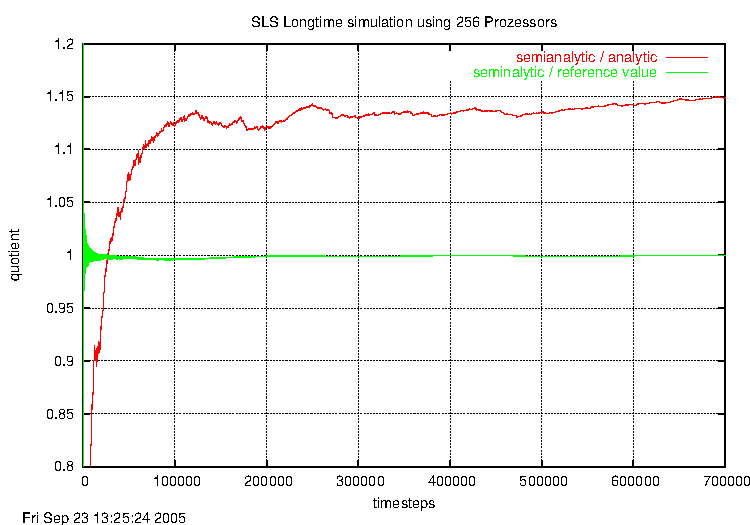
\includegraphics[width=0.80\textwidth]{sls-longterm.pdf}
   \caption{Longterm Behavior}
  \end{figure}
}


\section{Results of SLS-Simulation}
\frame {
  \frametitle{Results of SLS-Simulation}
  \begin{figure}[here]
  \centering
    \includegraphics[width=0.80\textwidth]{sls-acceptance.pdf}
   \caption{SLS-Acceptance vs. Touschek Lifetime}
  \end{figure}
}

\section{Low Emittance Study}
\frame {
  \frametitle{Simulation Results}
  \begin{figure}[here]
  \centering
    \includegraphics[width=0.80\textwidth]{emi.pdf}
   \caption{Low Emittance Studies}
  \end{figure}
}




\end{document}
